\documentclass{beamer}
\usepackage{amsmath}
\usepackage[utf8]{inputenc}
\usepackage{graphics}
\usepackage{hyperref}
\usepackage{xcolor}
\usepackage{wasysym}
\usepackage{listings}
\usepackage{tikz}
\usepackage{amssymb}
\usepackage[normalem]{ulem}
\usepackage{textcomp}
\usepackage{verbatim}
\usepackage[T1]{fontenc}
\usepackage{lmodern}
\usetikzlibrary{shapes.callouts,shadows, calc}

\tikzset{note/.style={rectangle callout, rounded corners,fill=gray!20,drop shadow,font=\footnotesize}}    
\newcommand{\tikzmark}[1]{\tikz[overlay,remember picture] \node (#1) {};}    

\newcounter{image}
\setcounter{image}{1}

\makeatletter
\newenvironment{btHighlight}[1][]
{\begingroup\tikzset{bt@Highlight@par/.style={#1}}\begin{lrbox}{\@tempboxa}}
{\end{lrbox}\bt@HL@box[bt@Highlight@par]{\@tempboxa}\endgroup}

\newcommand\btHL[1][]{%
  \begin{btHighlight}[#1]\bgroup\aftergroup\bt@HL@endenv%
}
\def\bt@HL@endenv{%
  \end{btHighlight}%   
  \egroup
}
\newcommand{\bt@HL@box}[2][]{%
  \tikz[#1]{%
    \pgfpathrectangle{\pgfpoint{0pt}{0pt}}{\pgfpoint{\wd #2}{\ht #2}}%
    \pgfusepath{use as bounding box}%
    \node[anchor=base west,rounded corners, fill=green!30,outer sep=0pt,inner xsep=0.2em, inner ysep=0.1em,  #1](a\theimage){\usebox{#2}};
  }%
 \stepcounter{image}
}
\makeatother

\usetheme{Warsaw}
\usecolortheme{lily}
\setbeamercovered{transparent}
\setbeamertemplate{headline}{
  \begin{beamercolorbox}{section in head/foot}
    \vskip2pt\insertnavigation{\paperwidth}\vskip2pt
  \end{beamercolorbox}
}

\setbeamertemplate{footline}{
}

\author{
  {\tiny Tony Morris\\}
}

\xdefinecolor{darkgreen}{rgb}{0,0.35,0}
\lstset{
  tabsize=2,
  basicstyle=\ttfamily,
  moredelim=**[is][\btHL]{`}{`}
}
\lstdefinelanguage{scala}{
  morekeywords={abstract,case,catch,class,def,%
    do,else,extends,false,final,finally,%
    for,forSome,if,implicit,import,lazy,match,%
    new,null,object,override,package,%
    private,protected,requires,return,sealed,%
    super,this,throw,trait,true,try,%
    type,val,var,while,with,yield},
  otherkeywords={=,=>,<-,<\%,<:,>:,\#,@},
  sensitive=true,
  morecomment=[l]{//},
  morecomment=[n]{/*}{*/},
  morestring=[b]",
  morestring=[b]',
  morestring=[b]"""
}
\lstdefinelanguage{haskell}{
  morekeywords={class,instance,where,do,data,newtype,default,deriving,module},
  otherkeywords={<-},
  sensitive=true,
  morecomment=[l]{--},
  morecomment=[n]{\{-}{-\}}, 
  morestring=[b]",
  morestring=[b]',
  morestring=[b]"""
}
\lstdefinelanguage{csharp}
{
  sensitive=true,
  morekeywords=[1]{
  abstract, as, base, break, case,
  catch, checked, class, const, continue,
  default, delegate, do, else, enum,
  event, explicit, extern, false,
  finally, fixed, for, foreach, goto, if,
  implicit, in, interface, internal, is,
  lock, namespace, new, null, operator,
  out, override, params, private,
  protected, public, readonly, ref,
  return, sealed, sizeof, stackalloc,
  static, struct, switch, this, throw,
  true, try, typeof, unchecked, unsafe,
  using, virtual, volatile, while, bool,
  byte, char, decimal, double, float,
  int, lock, object, sbyte, short, string,
  uint, ulong, ushort, void},
  morecomment=[l]{//},
  morecomment=[s]{/*}{*/},
  morecomment=[l][keywordstyle4]{\#},
  morestring=[b]",
  morestring=[b]',
}
\lstdefinestyle{java}{
  language=java,
  basicstyle=\footnotesize\ttfamily,
  stringstyle=\color{darkgreen}\ttfamily,
  commentstyle=\color{gray}\ttfamily,
  keywordstyle=\footnotesize\color{blue}\ttfamily,
  tabsize=2,
  moredelim=**[is][\btHL]{`}{`}
}
\lstdefinestyle{csharp}{
  language=csharp,
  basicstyle=\tiny\ttfamily,
  stringstyle=\color{darkgreen}\ttfamily,
  commentstyle=\color{gray}\ttfamily,
  keywordstyle=\tiny\color{blue}\ttfamily,
  tabsize=2,
  moredelim=**[is][\btHL]{`}{`}
}
\lstdefinestyle{scala}{
  language=scala,
  basicstyle=\footnotesize\ttfamily,
  stringstyle=\color{darkgreen}\ttfamily,
  commentstyle=\color{gray}\ttfamily,
  keywordstyle=\footnotesize\color{blue}\ttfamily,
  tabsize=2,
  moredelim=**[is][\btHL]{`}{`}
}
\lstdefinestyle{haskell}{
  language=haskell,
  basicstyle=\tiny\ttfamily,
  stringstyle=\color{darkgreen}\ttfamily,
  commentstyle=\color{gray}\ttfamily,
  keywordstyle=\tiny\color{blue}\ttfamily,
  tabsize=2
}
% #866eaa
\definecolor{nicta-purple}{rgb}{0.5234,0.4297,0.6640}

\defbeamertemplate*{title page}{customized}[1][] {
  \centering
  \color{nicta-purple}
  \usebeamerfont{title}\inserttitle\par
  \bigskip
  \usebeamerfont{subtitle}\insertsubtitle\par
  \bigskip
  \bigskip
  \bigskip
  \bigskip
  \usebeamerfont{institute}\insertinstitute\par
  \bigskip
  \usebeamerfont{author}\insertauthor\par
  % \usebeamerfont{date}\insertdate\par
  \usebeamercolor[fg]{titlegraphic}\inserttitlegraphic
}

\logo{
\includegraphics[height=0.8cm]{image/nicta.jpg}}

\begin{document}
\title{\large Functional Programming, Parametricity, Types}
\subtitle{\tiny Essential Tools of Programming}
\institute[NICTA]{}
\date {
  lca2016 FP Miniconf, 02 February 2016
}

\normalsize

\setbeamercovered{transparent}
\begin{frame}
  \titlepage
\end{frame}

\begin{frame}
\frametitle{The Premise}
\begin{block}{the following are essential to programming success\ldots}
\begin{itemize}
\item<1-> adherence to the functional programming thesis
\item<2-> parametricity (and types)
\end{itemize}
\end{block}
\end{frame}

\begin{frame}[fragile]
\frametitle{The Parametricity Trick}
\begin{block}{parametricity will only work with\ldots}
\begin{itemize}
\item<1-> an inveterate exploitation of the functional programming thesis
\item<2-> let's revisit functional programming
\end{itemize}
\end{block}
\end{frame}

\begin{frame}
\frametitle{Reminder}
\begin{block}{so what is functional programming?}
\begin{itemize}
\item<1-> a means of programming by which expressions are \emph{referentially transparent}.
\item<2-> but what is referential transparency?
\end{itemize}
\end{block}
\end{frame}

\begin{frame}
\frametitle{Referential Transparency}
\begin{itemize}
  \item<1-> referential transparency is a decidable property of program expressions
  \item<2-> functions provide programmers a tool to create referentially transparent expressions
\end{itemize}
\begin{block}<3>{The Test for Referential Transparency}
An expression \lstinline$expr$ is referentially transparent if in a program \lstinline$p$, all occurrences of \lstinline$expr$ in \lstinline$p$ can be replaced by an assignment to \lstinline$expr$ without effecting an observable change in \lstinline$p$.
\end{block}
\end{frame}

\begin{frame}[fragile]
\frametitle{Referential Transparency}
\begin{block}<1>{Example program}
\begin{lstlisting}
p = {
  r = buffer.append(x)
  r = buffer.append(x)
  f(r, r)
}
\end{lstlisting}
\end{block}
\begin{block}<2>{Refactoring of program}
\begin{lstlisting}
p = {
  f(buffer.append(x), buffer.append(x))
}
\end{lstlisting}
\end{block}
\begin{block}<3>{}
Is the program refactoring observable for all values of \lstinline$f$?
\end{block}
\end{frame}

\begin{frame}[fragile]
\frametitle{Referential Transparency}
\begin{block}<1>{Example program}
\begin{lstlisting}
p = {
  r = str.length()
  r = str.length()
  f(r, r)
}
\end{lstlisting}
\end{block}
\begin{block}<2>{Refactoring of program}
\begin{lstlisting}
p = {
  f(str.length(), str.length())
}
\end{lstlisting}
\end{block}
\begin{block}<3>{}
Is the program refactoring observable for all values of \lstinline$f$?
\end{block}
\end{frame}

\begin{frame}
\frametitle{Functional Programming}
\begin{itemize}
  \item<1-> FP is a commitment to preserving referential transparency
  \item<2-> Quite a while ago, FP won by not-a-little-bit.
  \item<3-> we use tools to achieve this commitment
  \item<4-> parametricity is one such tool with high reward
\end{itemize}
\end{frame}

\begin{frame}
\frametitle{What is Parametricity}
\begin{block}{Danielsson, Hughes, Jansson \& Gibbons \cite{danielsson2006fast} tell us:}
\begin{quotation}
Functional programmers often reason about programs as if
they were written in a total language, expecting the results
to carry over to non-total (partial) languages. We justify
such reasoning.
\end{quotation}
\end{block}
\end{frame}

\begin{frame}
\frametitle{What is Parametricity}
\begin{block}{Philip Wadler \cite{wadler1989theorems} tells us:}
\begin{quotation}
Write down the definition of a polymorphic function on a piece of paper. Tell me its type, but be careful not to let me see the function's definition. I will tell you a theorem that the function satisfies.

The purpose of this paper is to explain the trick.
\end{quotation}
\end{block}
\end{frame}

\begin{frame}[fragile]
\frametitle{Types}
\begin{block}{first let's talk about types}
Suppose we encountered the following function definition:
\begin{lstlisting}
int add12(int)
\end{lstlisting}
\end{block}
\begin{itemize}
  \item<1-> by the type alone, there are {$({2^{32}})^{2^{32}}$} possible implementations
  \item<2-> but this is a significantly smaller number than \rotatebox{90}{8}
\end{itemize}
\end{frame}

\begin{frame}[fragile]
\frametitle{Types}
\framesubtitle{reading the code}
We might form a suspicion that \lstinline[style=scala]$add12$ adds twelve to its argument
\begin{lstlisting}[style=scala]
int `add12`(int)
\end{lstlisting}
\begin{tikzpicture}[remember picture,overlay]
\coordinate (aa) at ($(a1)+(7,2.0)$);
\node[note,draw,callout relative pointer={($(aa)-(11.2,-3.7)$)},right] at (aa) {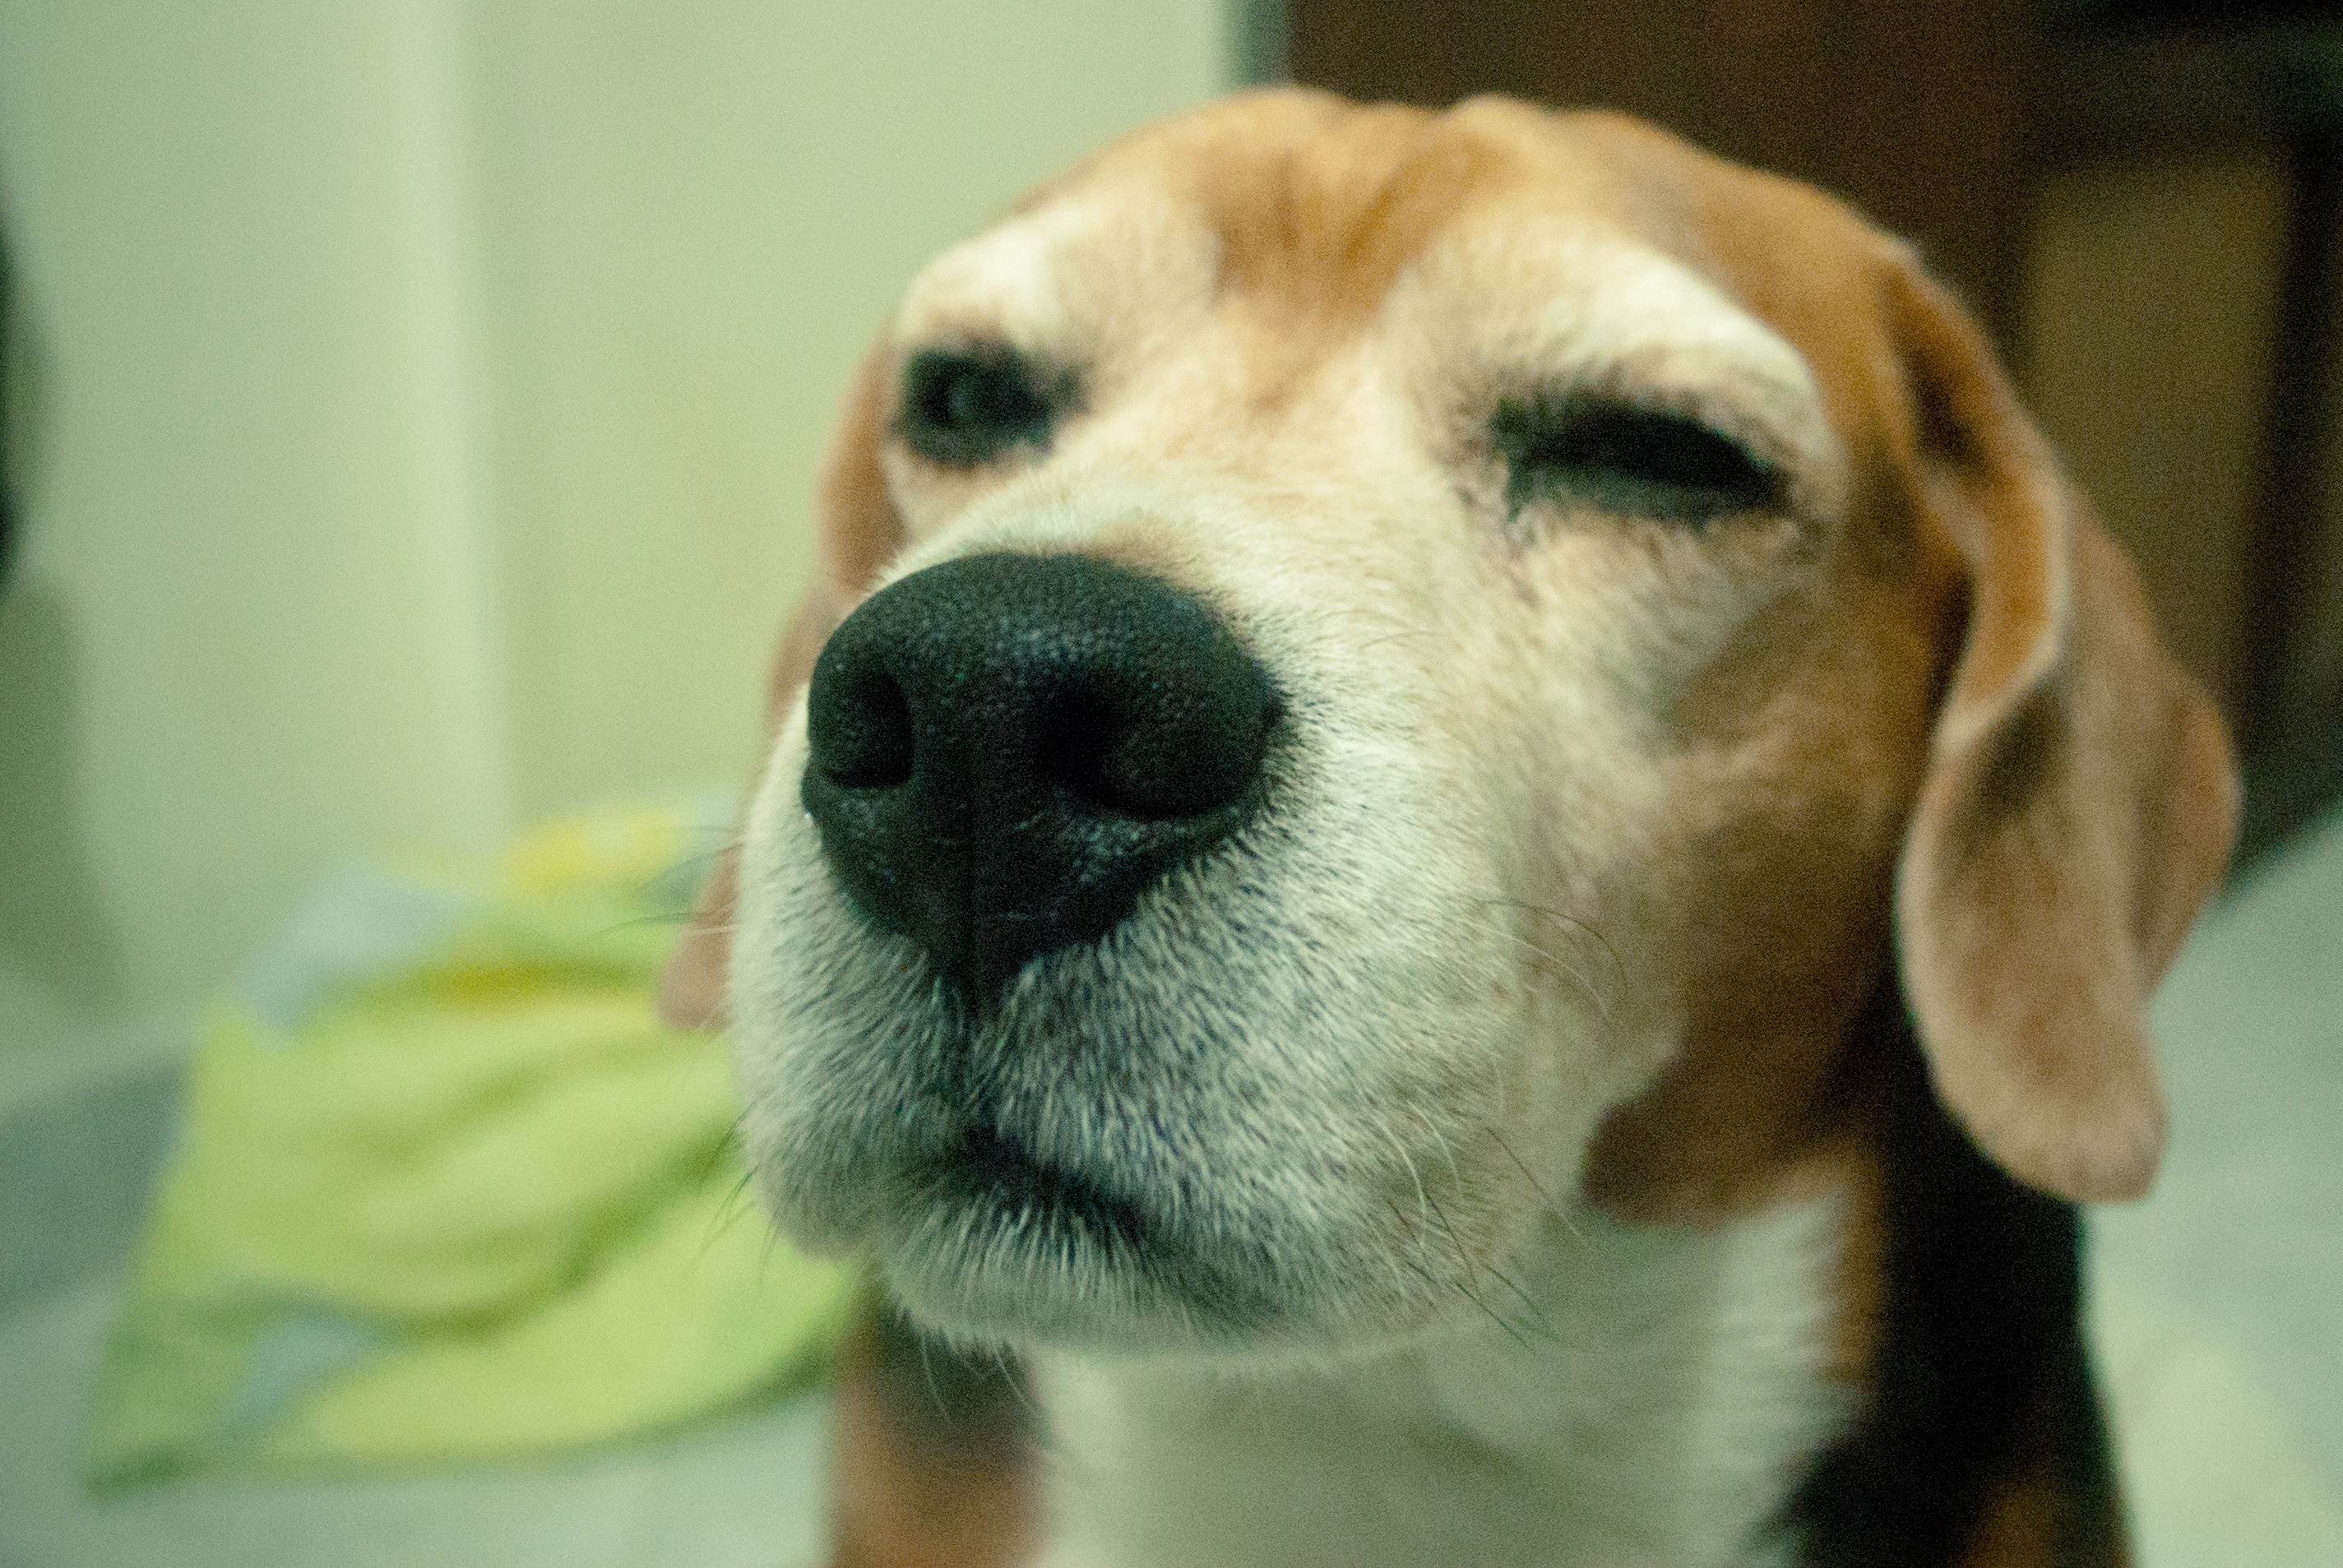
\includegraphics[width=0.2\textwidth]{image/suspicion.jpg}};
\end{tikzpicture}
\end{frame}

\begin{frame}[fragile]
\frametitle{Types}
So we write some tests:
\begin{lstlisting}
add12(0)        = 12
add12(5)        = 17
add12(-5)       = 7
add12(223)      = 235
add12(5096)     = 5104
add12(2914578)  = 29145590
add12(-2914578) = -29145566
\end{lstlisting}
And conclude, yes, this function adds twelve to its argument
\end{frame}

\begin{frame}[fragile]
\frametitle{Types}
\framesubtitle{Woops!}
\begin{lstlisting}
def add12(n: Int): Int =
  if(n < 8000000) n + 12
  else n * 7
\end{lstlisting}
Narrowing the potential propositions about what this function does not do.
\end{frame}

\begin{frame}[fragile]
\frametitle{Types}
\begin{block}{another monomorphic example}
\begin{lstlisting}
List<int> function(List<int>)
\end{lstlisting}
\end{block}
\begin{itemize}
  \item<1-> adds 17 to every 11th element?
  \item<2-> drops every prime number?
\end{itemize}
\end{frame}

\begin{frame}[fragile]
\frametitle{Parametricity}
\begin{block}{a polymorphic example}
\begin{lstlisting}
<A> List<A> function(List<A>)
\end{lstlisting}
\end{block}
\begin{itemize}
  \item<1-> this function returns elements in a list that always appear in the argument
  \item<2-> this function never inspects the elements, only rearranges them
\end{itemize}
\end{frame}

\begin{frame}[fragile]
\frametitle{Parametricity}
\begin{block}{the goal}
\begin{itemize}
  \item<1-> a significant number of possible things that this function does are eliminated, by no expenditure of effort
  \item<2-> theorems about this function can be reliably constructed
\end{itemize}
\end{block}
\end{frame}

\begin{frame}[fragile]
\frametitle{Reasoning with parametricity}
\begin{block}{Fast and loose reasoning is morally correct \cite{danielsson2006fast}}
\begin{quotation}
Functional programmers often reason about programs as if
they were written in a total language, expecting the results
to carry over to non-total (partial) languages. We justify
such reasoning.
\end{quotation}
\end{block}
but what does this mean exactly?
\end{frame}


\begin{frame}[fragile]
\frametitle{Fast and Loose Reasoning}
\begin{lstlisting}
boolean even(int i) =
  ...
\end{lstlisting}
We casually say, ``This function returns one of two things.''
\end{frame}

\begin{frame}[fragile]
\frametitle{Fast and Loose Reasoning}
\begin{lstlisting}
boolean even(int i) =
  even(i)
\end{lstlisting}
and we can discard this third possibility in analysis.
\end{frame}

\begin{frame}[fragile]
\frametitle{Fast and Loose Reasoning}
\begin{block}{many programming environments involve}
\begin{itemize}
  \item \lstinline{null}
  \item exceptions
  \item Type-casing
  \item Type-casting
  \item Side-effects \footnote{remember, FP has won, don't forget}
  \item universal \lstinline{equals}/\lstinline{toString}
\end{itemize}
\end{block}
These must \emph{all be discarded}. The penalty for this is \textbf{zero}.
\end{frame}

\begin{frame}[fragile]
\frametitle{The Limits of Parametricity}
\begin{block}{C\# type signature}
\begin{lstlisting}[style=csharp]
List<int> function(List<int>)
\end{lstlisting}
From the \emph{\textbf{monomorphic} type}, what does this function do?
\end{block}

\includegraphics[width=0.2\textwidth]{image/shrug.png}
\end{frame}

\begin{frame}[fragile]
\frametitle{The Limits of Parametricity}
\begin{block}{C\# type signature}
\begin{lstlisting}[style=csharp]
List<A> function<A>(List<A>)
\end{lstlisting}
From the \emph{\textbf{polymorphic} type}, what does this function do?
\end{block}
\large{\textbf{FACT: all elements in the result appear in the input.}}

\tiny{How do we narrow down to disambiguity?}
\end{frame}

\begin{frame}[fragile]
\frametitle{The Limits of Parametricity}
\begin{block}{Do we?}
\begin{itemize}
  \item<1-> write comments above the function

            \lstinline[style=csharp]{/* This function twiddles the database to twoddle out the twip twop */}

            \textbf{OR}
  \item<2-> write \emph{true} testable statements about the function
\end{itemize}
\end{block}
\end{frame}

\begin{frame}[fragile]
\frametitle{The Limits of Parametricity}
\begin{block}{what does this function do?}
\lstinputlisting[style=haskell]{source/reverse-with-tests.hs}
\end{block}
\end{frame}

\begin{frame}[fragile]
\frametitle{The Limits of Parametricity}
\begin{block}{what does this function do?}
\lstinputlisting[style=csharp,mathescape]{source/reverse-with-tests.cs}
\end{block}
\end{frame}

\begin{frame}[fragile]
\frametitle{The Limits of Parametricity}
\begin{block}{another example (Haskell)}
\begin{lstlisting}[style=haskell,mathescape]
flatMap :: (a -> List b) -> List a -> List b
flatMap = $\ldots$
\end{lstlisting}
\end{block}
\end{frame}

\begin{frame}[fragile]
\frametitle{The Limits of Parametricity}
\begin{block}{another example (C\#)}
\begin{lstlisting}[style=csharp,mathescape]
List<B> SelectMany<A, B>(this List<A>, Func<A, List<B>>) {
  $\ldots$
}
\end{lstlisting}
\end{block}
\end{frame}

\begin{frame}[fragile]
\frametitle{The Limits of Parametricity}
\begin{block}{another example}
\begin{lstlisting}[style=haskell,mathescape]
flatMap :: (a -> List b) -> List a -> List b
flatMap = $\ldots$
\end{lstlisting}
\begin{lstlisting}[style=csharp,mathescape]
List<B> SelectMany<A, B>(this List<A>, Func<A, List<B>>) {
  $\ldots$
}
\end{lstlisting}
\end{block}
\begin{itemize}
  \item If the input list is empty, so is the result
  \item Every \lstinline{(b)} in the result came from application of the given function
\end{itemize}
\end{frame}

\begin{frame}[fragile]
\frametitle{Once-inhabitance}
\begin{block}{sometimes tests are unnecessary}
\begin{lstlisting}[style=haskell]
f :: a -> a
\end{lstlisting}
\end{block}
\end{frame}

\begin{frame}[fragile]
\frametitle{Once-inhabitance}
\begin{block}{sometimes tests are unnecessary}
\begin{lstlisting}[style=haskell]
g :: Functor f => y -> f x -> f y
\end{lstlisting}
\end{block}
\emph{We already know that}
\begin{lstlisting}[style=haskell,mathescape]
$\lambda$> g "hi" [1,2,3]
["hi","hi","hi"]
\end{lstlisting}
\end{frame}

\begin{frame}[fragile]
\frametitle{Once-inhabitance}
\begin{block}{sometimes tests are \textbf{almost} unnecessary}
\begin{lstlisting}[style=haskell]
h :: a -> a -> a
\end{lstlisting}
\begin{lstlisting}[style=csharp]
A h<A>(A a1, A a2)
\end{lstlisting}
\end{block}
\end{frame}

\begin{frame}[fragile]
\frametitle{Once-inhabitance}
\begin{block}{sometimes tests are \textbf{almost} unnecessary}
\begin{lstlisting}[style=haskell]
h :: a -> a -> a
\end{lstlisting}
\begin{lstlisting}[style=csharp]
A h<A>(A a1, A a2)
\end{lstlisting}

\end{block}
\begin{lstlisting}[style=haskell,mathescape]
$\lambda$> h 7 8
7
\end{lstlisting}
\begin{lstlisting}[style=csharp]
csharp> h(7, 8)
7
\end{lstlisting}
\emph{We now know \textbf{precisely} what this function does}
\end{frame}

\begin{frame}[fragile]
\frametitle{Parametricity}
\begin{block}{non-trivial example}
\begin{lstlisting}[style=haskell]
both ::
  (Applicative f, Bitraversable r) =>
  (a -> f b) -> r a a -> f (r b b)
\end{lstlisting}
\end{block}
\tiny
\begin{itemize}
  \item<1-> This function can only \lstinline{bitraverse} \footnote{(and derivatives)} on \lstinline{(`r`)}
  \begin{itemize}
    \item \tiny{will work with \lstinline{Either} at call site}
    \item \tiny{will work with \lstinline{(,)} at call site}
    \item \tiny{will work with \lstinline{Const} at call site}
    \item \tiny{\textbf{but \lstinline{both} cannot do anything specific to these data types}}
  \end{itemize}
  \item<2-> This function can only \lstinline{(<*>)} and \lstinline{pure} on \lstinline{(`f`)}
  \begin{itemize}
    \item \tiny{will work with \lstinline{Maybe} at call site}
    \item \tiny{will work with \lstinline{IO} at call site}
    \item \tiny{e.g. call site can open network connections using \lstinline{both}}
    \item \tiny{\textbf{however \lstinline{both} definitely does not open any network connections itself}}
  \end{itemize}
  \item<3-> \lstinline{(`a`)} and \lstinline{(`b`)} might be anything
  \begin{itemize}
    \item \tiny{may be \lstinline{Int} at call site}
    \item \tiny{may be \lstinline{String} at call site}
    \item \tiny{\textbf{however \lstinline{both} definitely does not perform any \lstinline{Int}-specific operations}}
  \end{itemize}
\end{itemize}
\end{frame}

\begin{frame}[fragile]
\frametitle{Parametricity}
\begin{block}{and on it goes}
\begin{lstlisting}[style=haskell]
(<.) ::
  Indexable i p =>
  (Indexed i s t -> r) -> ((a -> b) -> s -> t) -> p a b -> r
\end{lstlisting}
\end{block}
\end{frame}

\begin{frame}[fragile]
\frametitle{Code readability}
\begin{block}{hang on a minute}
Did you just work out what that code did, by using types?
\end{block}
\end{frame}

\begin{frame}[fragile]
\frametitle{Code readability}
\begin{block}{Yes, yes I did}
Types are documentation
\end{block}
\end{frame}

\begin{frame}[fragile]
\frametitle{Code readability}
\begin{block}{Types are documentation}
\emph{reliable and dense documentation}
\end{block}
\end{frame}

\begin{frame}[fragile]
\frametitle{Code readability}
\begin{block}{Reliable documentation}
\emph{like comments, except condensed, machine-checked, without the fluff and falsehoods}
\end{block}
\end{frame}

\begin{frame}[fragile]
\frametitle{Parametricity, practical goals}
\begin{block}{typical software development goals}
\begin{itemize}
  \item<1-> can fix bugs independently of the possibility of creating more
  \item<2-> can introduce features without adversely affecting others
  \item<3-> can have hundreds of projects requiring zero maintenance
  \item<4-> can reliably and efficiently determine what goal existing code achieves
  \item<5-> \textbf{avoid endless tail-chasing that prevails in corporate dev}
\end{itemize}
\end{block}
\end{frame}

\begin{frame}[fragile]
\frametitle{Parametricity, practical goals}
\begin{block}{anti-goals}
\begin{quotation}
The Marine Corps' F-35B aircraft are being delivered with Block 2B software, which Gilmore said has ``hundreds of unresolved deficiencies.'' And those problems have compounded in Block 3F software. That's because the first round of Block 3 was created by ``re-hosting the immature Block 2B software…into new processors to create Block 3i,'' the initial release for the code, Gilmore noted. This led to ``avionics instabilities and other new problems, resulting in poor performance during developmental testing.''
\end{quotation}
\end{block}
\begin{center}
\textbf{DO NOT WANT TO BE HERE}
\end{center}
\end{frame}

\begin{frame}[fragile]
\frametitle{Parametricity, practical goals}
\begin{block}{common questions pertaining to goals}
\begin{itemize}
  \item what tools assist in achieving these goals?
  \item what tools do we know do not achieve these goals?
\end{itemize}
\end{block}
\end{frame}

\begin{frame}[fragile]
\frametitle{Parametricity, practical goals}
\begin{block}{common snarks distracting from goals}
\begin{itemize}
  \item what's it like for you haskell programmers in the ivory tower?
  \item why do you hate programming language environment X?
  \item ``but all tools have a job for which they are suited''
  \item why are you so fundamentalist?
  \item why are you so extweemust?
\end{itemize}
\end{block}
\end{frame}

\begin{frame}[fragile]
\frametitle{Parametricity, practical goals}
\begin{block}{goals}
``Here is programming language environment X, which undermines your capability to exploits types and parametricity.''
\end{block}
\textbf{for what benefit?}
\end{frame}

\begin{frame}[fragile]
\frametitle{Parametricity, practical goals}
\begin{block}{goals}
Propose to forgo these practical tools, and a reasonable compromise must be substituted, else dismissal
\end{block}
\end{frame}

\begin{frame}[fragile]
\frametitle{Parametricity, practical goals}
\begin{block}{goals}
You may one day be persuaded that this is an unreasonable approach to your objective.
\end{block}
\begin{center}
\textbf{IT'S A MIND TRAP}
\end{center}
\end{frame}

\begin{frame}[fragile]
\frametitle{Parametricity, practical goals}
\begin{block}{goals}
Parametricity is for winners who achieve their goals.

Let's all be winners.
\end{block}
\begin{center}
\textbf{\emph{Spread the polymorphic love.}}
\end{center}
\end{frame}

\begin{frame}
\frametitle{References}

\bibliographystyle{amsalpha}
\bibliography{parametricity}

\end{frame}


\end{document}
